% https://www.sharelatex.com/blog/2013/08/27/tikz-series-pt1.html

\documentclass[tikz]{standalone}

\begin{document}
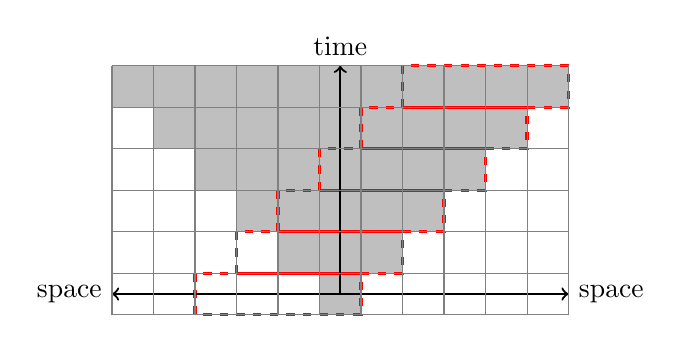
\begin{tikzpicture}[x=1.5em,y=1.5em]
  \fill[lightgray] (0,5) rectangle (11, 6);
  \fill[lightgray] (1,4) rectangle (10, 5);
  \fill[lightgray] (2,3) rectangle (9, 4);
  \fill[lightgray] (3,2) rectangle (8, 3);
  \fill[lightgray] (4,1) rectangle (7, 2);
  \fill[lightgray] (5,0) rectangle (6, 1);

  \onslide<2> {
    \foreach \ts in {0,...,5} {
      \draw[very thick, dashed, red] (\ts+2,\ts) rectangle (\ts+6,\ts+1);
     }
  }

  \draw[thick,->] (5.5,0.5) -- (5.5, 6) node (yaxis) [above] {time}; 
  \draw[thick, <->] (0,0.5) node [left] {space} -- (11,0.5) node (xaxis) [right] {space};
  \draw[gray, step=1] (0,0) grid (11,6);
\end{tikzpicture}
\end{document}
